\documentclass[a4paper]{article}
\usepackage[utf8]{inputenc}
\usepackage[spanish, es-tabla, es-noshorthands]{babel}
\usepackage[table,xcdraw]{xcolor}
\usepackage[a4paper, footnotesep=1.25cm, headheight=1.25cm, top=2.54cm, left=2.54cm, bottom=2.54cm, right=2.54cm]{geometry}
%\geometry{showframe}

%\usepackage{wrapfig}			%Wrap figure in text
\usepackage[export]{adjustbox}	%Move images
\usepackage{changepage}			%Move tables

\usepackage{tikz}
\usepackage{amsmath}
\usepackage{amsfonts}
\usepackage{amssymb}
\usepackage{float}
\usepackage{graphicx}
\usepackage{caption}
\usepackage{subcaption}
\usepackage{multicol}
\usepackage{multirow}
\usepackage{wrapfig}
\setlength{\doublerulesep}{\arrayrulewidth}
\usepackage{booktabs}
\usepackage[numbib, nottoc, notlot, notlof]{tocbibind}

\usepackage{hyperref}
\hypersetup{
    colorlinks=true,
    linkcolor=blue,
    filecolor=magenta,      
    urlcolor=blue,
    citecolor=blue,    
}

%Change Font Size

% #1 = size, #2 = text
\newcommand{\setparagraphsize}[2]{{\fontsize{#1}{6}\selectfont#2 \par}}		%Cambia el size de todo el parrafo
\newcommand{\setlinesize}[2]{{\fontsize{#1}{6}\selectfont#2}}				%Cambia el font de una oración

\newcommand{\note}[1]{
	\begin{center}
		\huge{ \textcolor{red}{#1} }
	\end{center}
}

%FONTS (IMPORTANTE): Compilar en XeLaTex o LuaLaTeX
\usepackage{anyfontsize}	%Font size
\usepackage{fontspec}		%Font type

\usepackage{etoolbox}
\usepackage{todonotes}

\newcommand{\observacion}[2]{  \ifnumequal{1}{#1}{ { \todo[inline,backgroundcolor=red!25,bordercolor=red!100]{\textbf{Observación: #2}} } }{  }  }

\setcounter{topnumber}{2}
\setcounter{bottomnumber}{2}
\setcounter{totalnumber}{4}
\renewcommand{\topfraction}{0.85}
\renewcommand{\bottomfraction}{0.85}
\renewcommand{\textfraction}{0.15}
\renewcommand{\floatpagefraction}{0.8}
\renewcommand{\textfraction}{0.1}
\setlength{\floatsep}{5pt plus 2pt minus 2pt}
\setlength{\textfloatsep}{5pt plus 2pt minus 2pt}
\setlength{\intextsep}{5pt plus 2pt minus 2pt}

\newcommand{\quotes}[1]{``#1''}
\usepackage{array}
\newcolumntype{C}[1]{>{\centering\let\newline\\\arraybackslash\hspace{0pt}}m{#1}}
\usepackage[american]{circuitikz}
\usetikzlibrary{calc}
\usepackage{fancyhdr}
\usepackage{units} 

\graphicspath{{../Control de posición no lineal/}{../Control de fuerza no lineal/}{../Control híbrido no lineal/}{../Referencias/}{../Deducción de modelo/}{../Conclusiones/}}

\pagestyle{fancy}
\fancyhf{}
\lhead{22.99 - Automación Industrial}
\rhead{Lambertucci, Londero B., Maselli, Mechoulam}
\rfoot{Página \thepage}

%Items con bullets y no cuadrados
\renewcommand{\labelitemi}{\textbullet }


\begin{document}

%%%%%%%%%%%%%%%%%%%%%%%%%
%		Caratula		%
%%%%%%%%%%%%%%%%%%%%%%%%%

%\setmainfont{Avenir LT Std 55 Roman}
\setmainfont{AvenirLTStd-Roman}

\begin{titlepage}

\begin{tikzpicture}[remember picture, overlay, black, line width = 0.5pt]
	\coordinate (a) at (-2cm,2cm);
	\coordinate (b) at (17cm,-25.5cm);
	
	\coordinate (ap) at (-2.1cm,2.1cm);
	\coordinate (bp) at (17.1cm,-25.6cm);
	
	\draw[] (a) -| (b);
	\draw[] (a) |- (b);
	
	\draw[] (ap) -| (bp);
	\draw[] (ap) |- (bp);
	
	%footnotesep=1.25cm, headheight=1.25cm, top=2.54cm, left=2.54cm, bottom=2.54cm, right=2.54cm

\end{tikzpicture}

\begin{figure}[H]
	
\includegraphics[width=0.3\linewidth, right]{./Utils/ITBA_1}
\end{figure}

\vspace*{1.5cm}

\noindent \textbf{\setlinesize{12}{INSTITUTO TECNOLÓGICO DE BUENOS AIRES - ITBA}}

\noindent \textbf{\setlinesize{12}{ESCUELA DE INGENIERÍA Y TECNOLOGÍA}}

\vspace*{4cm}

\begin{center}
	\setlinesize{24}{ \textbf{TRABAJO PRÁCTICO FINAL} }
	
	\vspace*{1.5cm}
	%\setlinesize{24}{ \textbf{Subtítulo del trabajo (cuando corresponda)} }
	\vspace*{1.0cm}
\end{center}
\begin{center}
	\setlinesize{18}{ \textbf{MANUAL DE USUARIO} }
	
	\vspace*{1.5cm}
	%\setlinesize{24}{ \textbf{Subtítulo del trabajo (cuando corresponda)} }
	\vspace*{1.0cm}
\end{center}
\begin{figure}[H]
\begin{adjustwidth}{-1cm}{}
\begin{tabular}{llr} 
	\textbf{AUTORES:}
	& \textbf{Lambertucci, Guido Enrique} & \textbf{(Leg. N}$\mathbf{^o}$ \textbf{58009)} \\
	& \textbf{Londero Bonaparte, Tomás Guillermo} & \textbf{(Leg. N}$\mathbf{^o}$ \textbf{58150)} \\
	& \textbf{Mechoulam, Alan}  &  \textbf{(Leg. N}$\mathbf{^o}$ \textbf{58438)}\\
	& \textbf{Maselli, Carlos Javier} &  \textbf{(Leg. N}$\mathbf{^o}$ \textbf{59564)} \\
	 
 &  & \\
 &  & \\
	\textbf{DOCENTES}:
	& \textbf{Arias, Rodolfo Enrique} & \\
	& \textbf{Sofio Avogadro, Federico} & \\
	& \textbf{Spinelli, Mariano Tomás} & \\
\end{tabular}
\end{adjustwidth}
\end{figure}

\vspace*{0.5cm}
\center{
%{\noindent \setparagraphsize{12}{\textbf{TRABAJO PRÁCTICO N$^{\circ}$1}}}
{\noindent \setparagraphsize{12}{\textbf{\textsc{22.90 - Automación Industrial}}}}
}
\vspace*{1.5cm}

\center{\textbf{BUENOS AIRES}}

\end{titlepage}


\setmainfont{Calibri}

%%%%%%%%%%%%%%%%%%%%%
%		Indice		%
%%%%%%%%%%%%%%%%%%%%%

\tableofcontents
\newpage

%%%%%%%%%%%%%%%%%%%%%
%		Informe		%
%%%%%%%%%%%%%%%%%%%%%

\section{Deducción de modelo}
%\documentclass[a4paper]{article}
\usepackage[utf8]{inputenc}
\usepackage[spanish, es-tabla, es-noshorthands]{babel}
\usepackage[table,xcdraw]{xcolor}
\usepackage[a4paper, footnotesep=1.25cm, headheight=1.25cm, top=2.54cm, left=2.54cm, bottom=2.54cm, right=2.54cm]{geometry}
%\geometry{showframe}

%\usepackage{wrapfig}			%Wrap figure in text
\usepackage[export]{adjustbox}	%Move images
\usepackage{changepage}			%Move tables

\usepackage{tikz}
\usepackage{amsmath}
\usepackage{amsfonts}
\usepackage{amssymb}
\usepackage{float}
\usepackage{graphicx}
\usepackage{caption}
\usepackage{subcaption}
\usepackage{multicol}
\usepackage{multirow}
\usepackage{wrapfig}
\setlength{\doublerulesep}{\arrayrulewidth}
\usepackage{booktabs}
\usepackage[numbib, nottoc, notlot, notlof]{tocbibind}

\usepackage{hyperref}
\hypersetup{
    colorlinks=true,
    linkcolor=blue,
    filecolor=magenta,      
    urlcolor=blue,
    citecolor=blue,    
}

%Change Font Size

% #1 = size, #2 = text
\newcommand{\setparagraphsize}[2]{{\fontsize{#1}{6}\selectfont#2 \par}}		%Cambia el size de todo el parrafo
\newcommand{\setlinesize}[2]{{\fontsize{#1}{6}\selectfont#2}}				%Cambia el font de una oración

\newcommand{\note}[1]{
	\begin{center}
		\huge{ \textcolor{red}{#1} }
	\end{center}
}

%FONTS (IMPORTANTE): Compilar en XeLaTex o LuaLaTeX
\usepackage{anyfontsize}	%Font size
\usepackage{fontspec}		%Font type

\usepackage{etoolbox}
\usepackage{todonotes}

\newcommand{\observacion}[2]{  \ifnumequal{1}{#1}{ { \todo[inline,backgroundcolor=red!25,bordercolor=red!100]{\textbf{Observación: #2}} } }{  }  }

\setcounter{topnumber}{2}
\setcounter{bottomnumber}{2}
\setcounter{totalnumber}{4}
\renewcommand{\topfraction}{0.85}
\renewcommand{\bottomfraction}{0.85}
\renewcommand{\textfraction}{0.15}
\renewcommand{\floatpagefraction}{0.8}
\renewcommand{\textfraction}{0.1}
\setlength{\floatsep}{5pt plus 2pt minus 2pt}
\setlength{\textfloatsep}{5pt plus 2pt minus 2pt}
\setlength{\intextsep}{5pt plus 2pt minus 2pt}

\newcommand{\quotes}[1]{``#1''}
\usepackage{array}
\newcolumntype{C}[1]{>{\centering\let\newline\\\arraybackslash\hspace{0pt}}m{#1}}
\usepackage[american]{circuitikz}
\usetikzlibrary{calc}
\usepackage{fancyhdr}
\usepackage{units} 

\graphicspath{{../Control de posición no lineal/}{../Control de fuerza no lineal/}{../Control híbrido no lineal/}{../Referencias/}{../Deducción de modelo/}{../Conclusiones/}}

\pagestyle{fancy}
\fancyhf{}
\lhead{22.99 - Automación Industrial}
\rhead{Lambertucci, Londero B., Maselli, Mechoulam}
\rfoot{Página \thepage}

%Items con bullets y no cuadrados
\renewcommand{\labelitemi}{\textbullet }


%\begin{document}

\subsection{XXX}

%\end{document}


\section{Control de posición no lineal}
%\documentclass[a4paper]{article}
\usepackage[utf8]{inputenc}
\usepackage[spanish, es-tabla, es-noshorthands]{babel}
\usepackage[table,xcdraw]{xcolor}
\usepackage[a4paper, footnotesep=1.25cm, headheight=1.25cm, top=2.54cm, left=2.54cm, bottom=2.54cm, right=2.54cm]{geometry}
%\geometry{showframe}

%\usepackage{wrapfig}			%Wrap figure in text
\usepackage[export]{adjustbox}	%Move images
\usepackage{changepage}			%Move tables

\usepackage{tikz}
\usepackage{amsmath}
\usepackage{amsfonts}
\usepackage{amssymb}
\usepackage{float}
\usepackage{graphicx}
\usepackage{caption}
\usepackage{subcaption}
\usepackage{multicol}
\usepackage{multirow}
\usepackage{wrapfig}
\setlength{\doublerulesep}{\arrayrulewidth}
\usepackage{booktabs}
\usepackage[numbib, nottoc, notlot, notlof]{tocbibind}

\usepackage{hyperref}
\hypersetup{
    colorlinks=true,
    linkcolor=blue,
    filecolor=magenta,      
    urlcolor=blue,
    citecolor=blue,    
}

%Change Font Size

% #1 = size, #2 = text
\newcommand{\setparagraphsize}[2]{{\fontsize{#1}{6}\selectfont#2 \par}}		%Cambia el size de todo el parrafo
\newcommand{\setlinesize}[2]{{\fontsize{#1}{6}\selectfont#2}}				%Cambia el font de una oración

\newcommand{\note}[1]{
	\begin{center}
		\huge{ \textcolor{red}{#1} }
	\end{center}
}

%FONTS (IMPORTANTE): Compilar en XeLaTex o LuaLaTeX
\usepackage{anyfontsize}	%Font size
\usepackage{fontspec}		%Font type

\usepackage{etoolbox}
\usepackage{todonotes}

\newcommand{\observacion}[2]{  \ifnumequal{1}{#1}{ { \todo[inline,backgroundcolor=red!25,bordercolor=red!100]{\textbf{Observación: #2}} } }{  }  }

\setcounter{topnumber}{2}
\setcounter{bottomnumber}{2}
\setcounter{totalnumber}{4}
\renewcommand{\topfraction}{0.85}
\renewcommand{\bottomfraction}{0.85}
\renewcommand{\textfraction}{0.15}
\renewcommand{\floatpagefraction}{0.8}
\renewcommand{\textfraction}{0.1}
\setlength{\floatsep}{5pt plus 2pt minus 2pt}
\setlength{\textfloatsep}{5pt plus 2pt minus 2pt}
\setlength{\intextsep}{5pt plus 2pt minus 2pt}

\newcommand{\quotes}[1]{``#1''}
\usepackage{array}
\newcolumntype{C}[1]{>{\centering\let\newline\\\arraybackslash\hspace{0pt}}m{#1}}
\usepackage[american]{circuitikz}
\usetikzlibrary{calc}
\usepackage{fancyhdr}
\usepackage{units} 

\graphicspath{{../Control de posición no lineal/}{../Control de fuerza no lineal/}{../Control híbrido no lineal/}{../Referencias/}{../Deducción de modelo/}{../Conclusiones/}}

\pagestyle{fancy}
\fancyhf{}
\lhead{22.99 - Automación Industrial}
\rhead{Lambertucci, Londero B., Maselli, Mechoulam}
\rfoot{Página \thepage}

%Items con bullets y no cuadrados
\renewcommand{\labelitemi}{\textbullet }


%\begin{document}

\subsection{Caracterizaci\'on del problema}
Se pide un control cartesiano no lineal para el manipulador RR. Agregando una zona prohibida que es todo valor por encima de una pared, descrita en el plano XY pro la siguiente ecuaci\'on:
\begin{equation}
y=2-x
\end{equation}
Al manipulador se le pide que vaya del punto (1;-1;0) a (1;1;0). Para generar la trayectoria se utiliza la función \textbf{jtraj} del toolbox de matlab de Peter Corke.
\subsection{Esquema de control}
El modelo de control porpuesto es el conocido como linealizaci\'on por realimentaci\'on.
Es fundamental para este tipo de control tener un gran conocimiento de la planta, ya que basicamente se lo controla como si fuese lineal, con un esquema tipo PD. Con la diferencia que se le agrega  a la acci\'on de control la respuesta no lineal de la planta, gracias al conocimiento del modelo no lineal de la planta y sus variables de estado.
\begin{figure}[H]
	\centering
	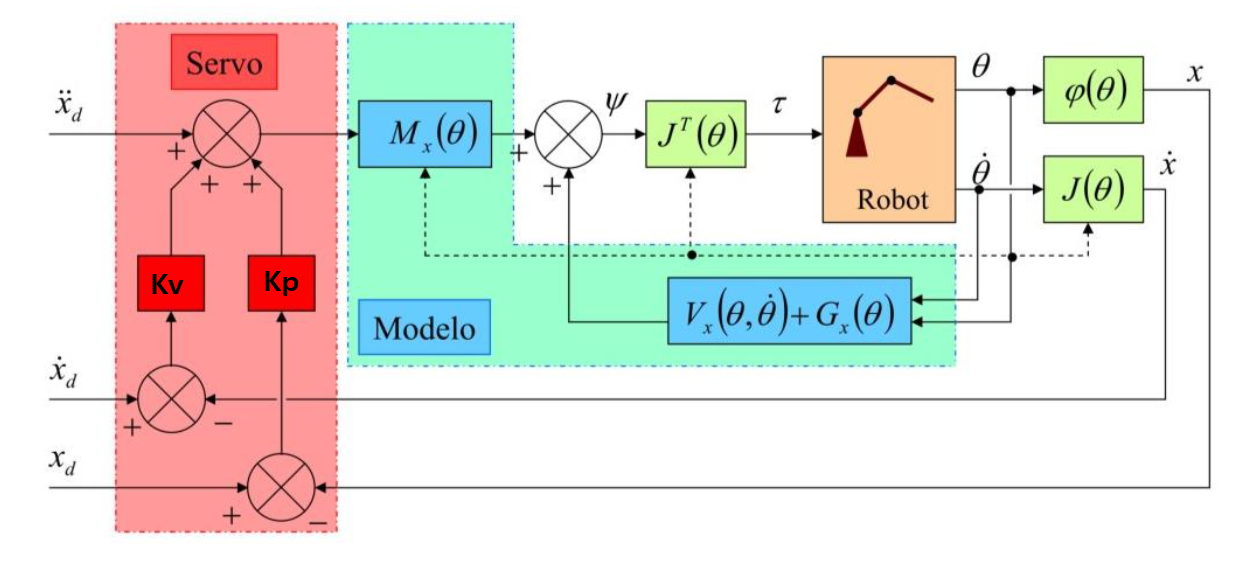
\includegraphics[width=0.8\linewidth]{ImagenesControl de posición no lineal/modelo_control_p}
	\caption{Topolog\'ia del control de posici\'on cartesiano no lineal.}	
	\label{fig:control_p_modelo}
\end{figure}
Cabe mencionar que las matrices $M_x,\ V_x, \ y \ G_x$ se encuentran en espacio cartesiano, y la manera de pasar de las mismas en espacio joint es la siguiente:
\begin{equation}
M_x(\Theta) = J^{-T}(\Theta) M(\Theta) J^{-1}(\Theta)
\end{equation} 
\begin{equation}
V_x(\Theta , \dot{\Theta}) = J^{-T}(\Theta) \left( V(\Theta , \dot{\Theta}) - M(\Theta) J^{-1}(\Theta) \dot{J}(\Theta) \dot{\Theta} \right)
\end{equation} 
\begin{equation}
G_x(\Theta) = J^{-T}(\Theta) G(\Theta) 
\end{equation}


HABLAR DE VALROES DE GANANCIAS

\subsection{Resultados}
Se realiz\'o el simulink del sistema. Obteniendo los siguientes gr\'aficos.
Aqui se pueden observar los angulos de los manipuladores en espacio de joint.
Como el primer rotacional hace una trayectoria de $-\frac{\pi}{2}$ hacia 0, y el segundo si bien el punto inicial y final son el mismo, se desv\'ia con el prop\'osito de seguir la trayectoria cartesiana indicada.
\begin{figure}[H]
	\centering
	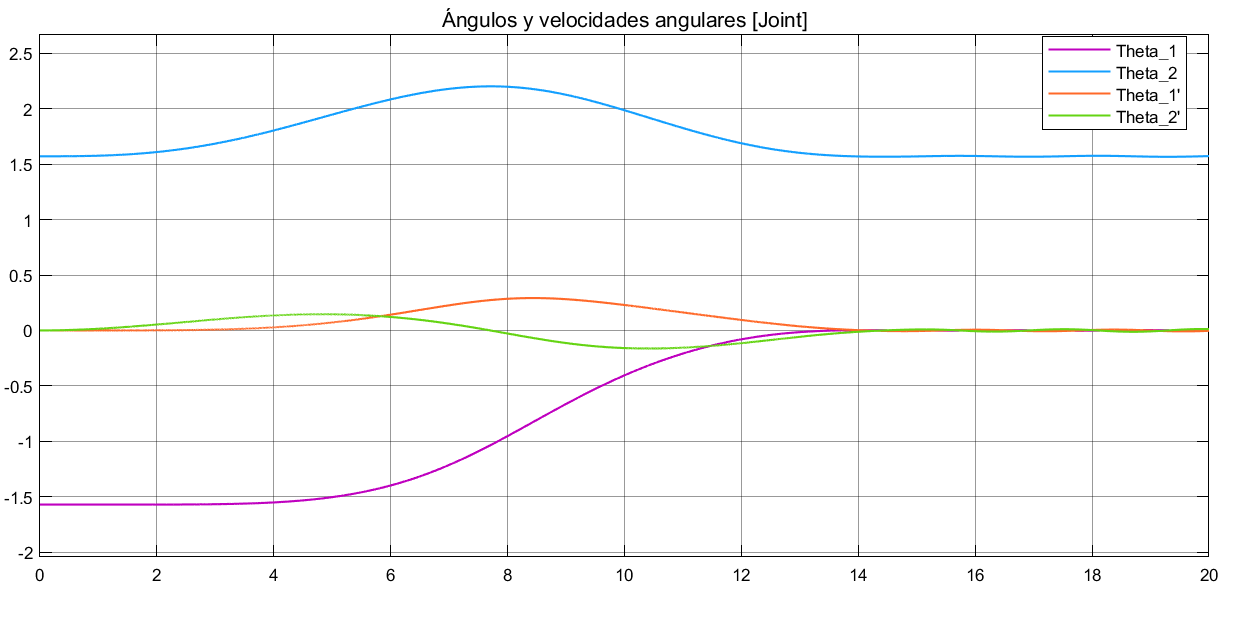
\includegraphics[width=0.8\linewidth]{ImagenesControl de posición no lineal/1_3_a}
	\caption{\'Angulos en funci\'on del tiempo en espacio joint.}	
	\label{fig:athetas}
\end{figure}
Aqu\'i se ven tanto las referencias como las coordendas reales que tomo el EE, con un error porcentual menor al XX$\%$ 
\begin{figure}[H]
	\centering
	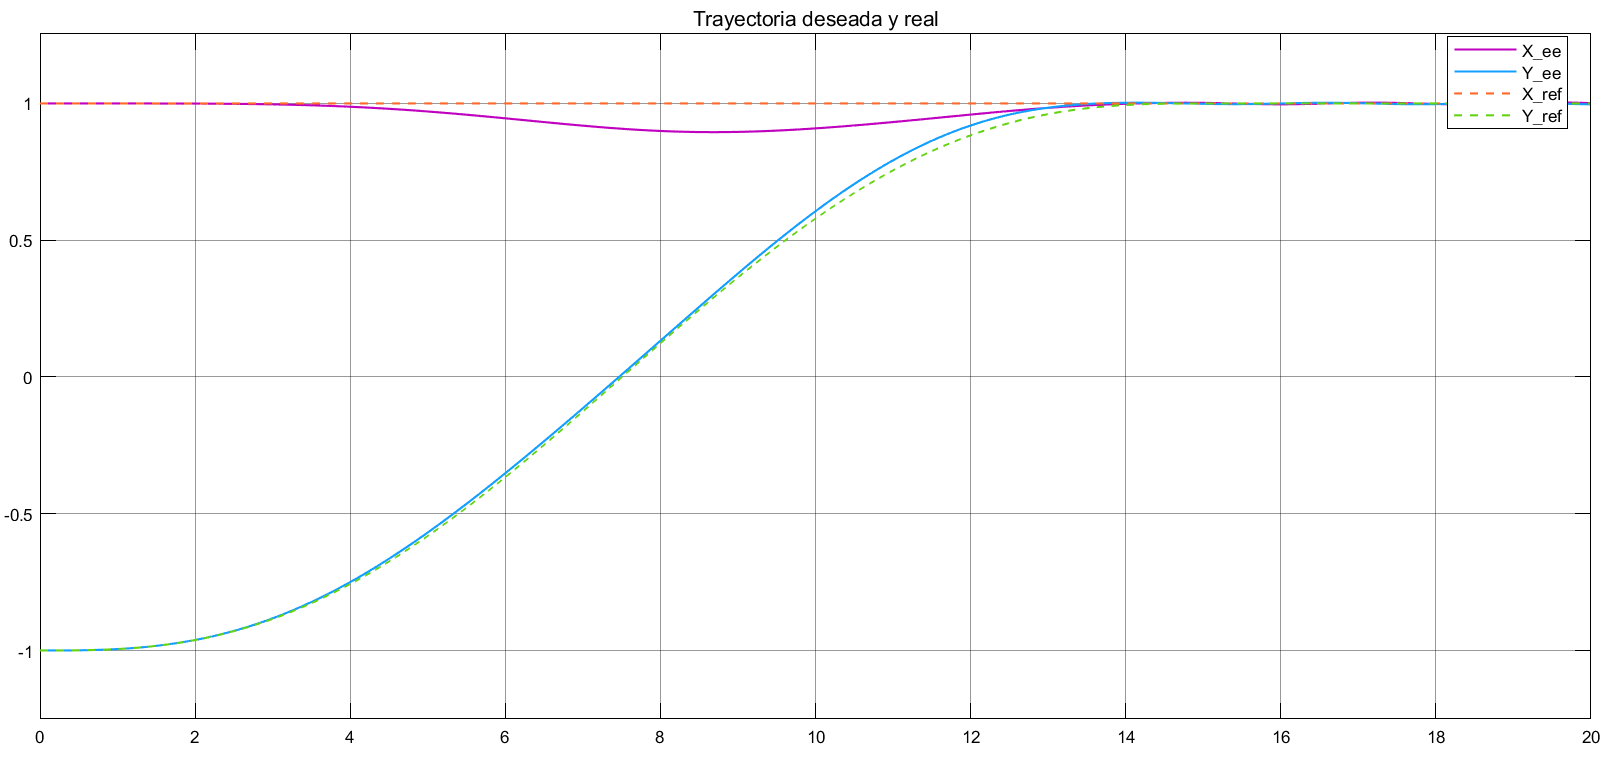
\includegraphics[width=0.8\linewidth]{ImagenesControl de posición no lineal/1_3_b}
	\caption{Posici\'on deseada y real del EE.}	
	\label{fig:apos}
\end{figure}

La trayectoria descripta por el EE se observa claramente en la siguiente imagen.
\begin{figure}[H]
	\centering
	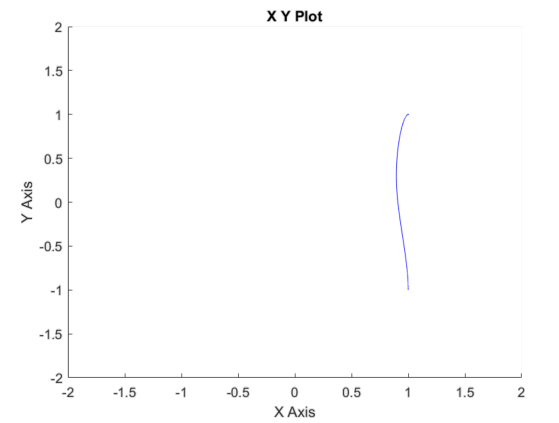
\includegraphics[width=0.5\linewidth]{ImagenesControl de posición no lineal/1_3_c}
	\caption{Gr\'afico XY.}	
	\label{fig:axy}
\end{figure}

Ademas se le incluy\'o un disturbio a la planta tanto en posici\'on como en velocidad. Este disturbio sucede en el segundo 14. Y se observa en los siguientes gráficos como el manipulador se ve afectado por el mismo y luego vuelve rápidamente a la referencia.

\begin{figure}[H]
	\centering
	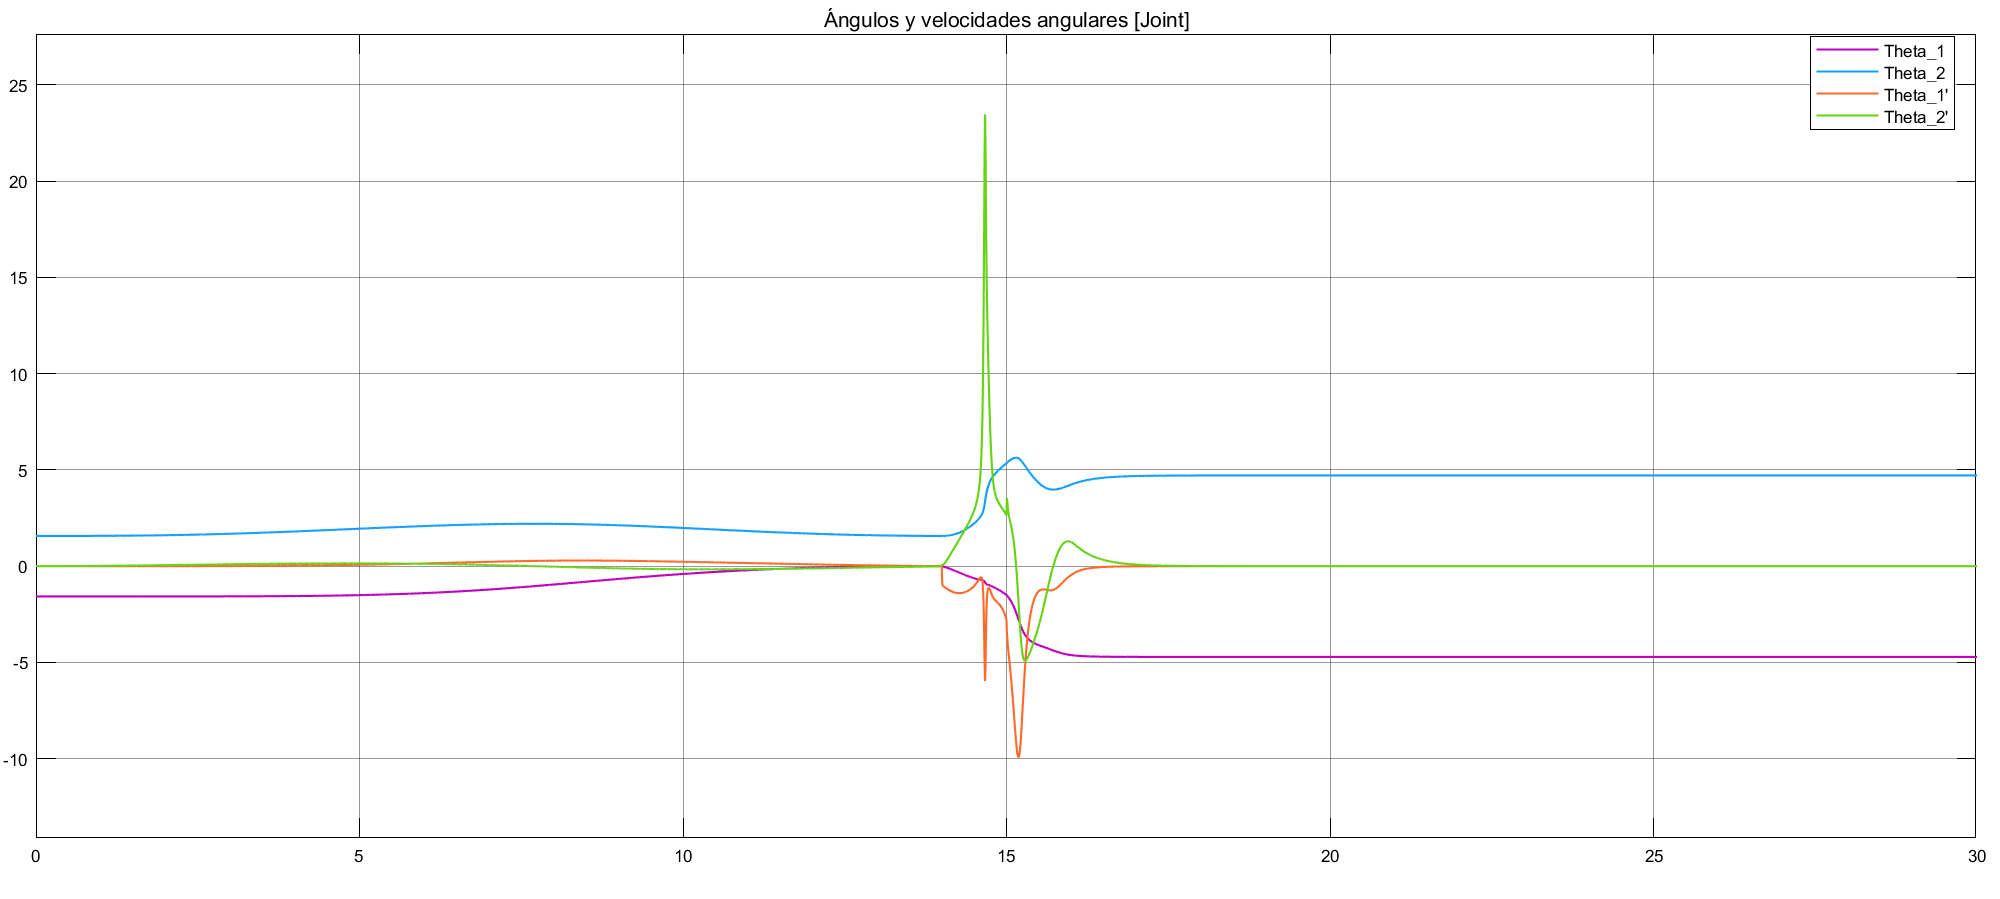
\includegraphics[width=0.8\linewidth]{ImagenesControl de posición no lineal/1_3_e_a}
	\caption{\'Angulos en funci\'on del tiempo en espacio joint.}	
	\label{fig:athetasd}
\end{figure}

\begin{figure}[H]
	\centering
	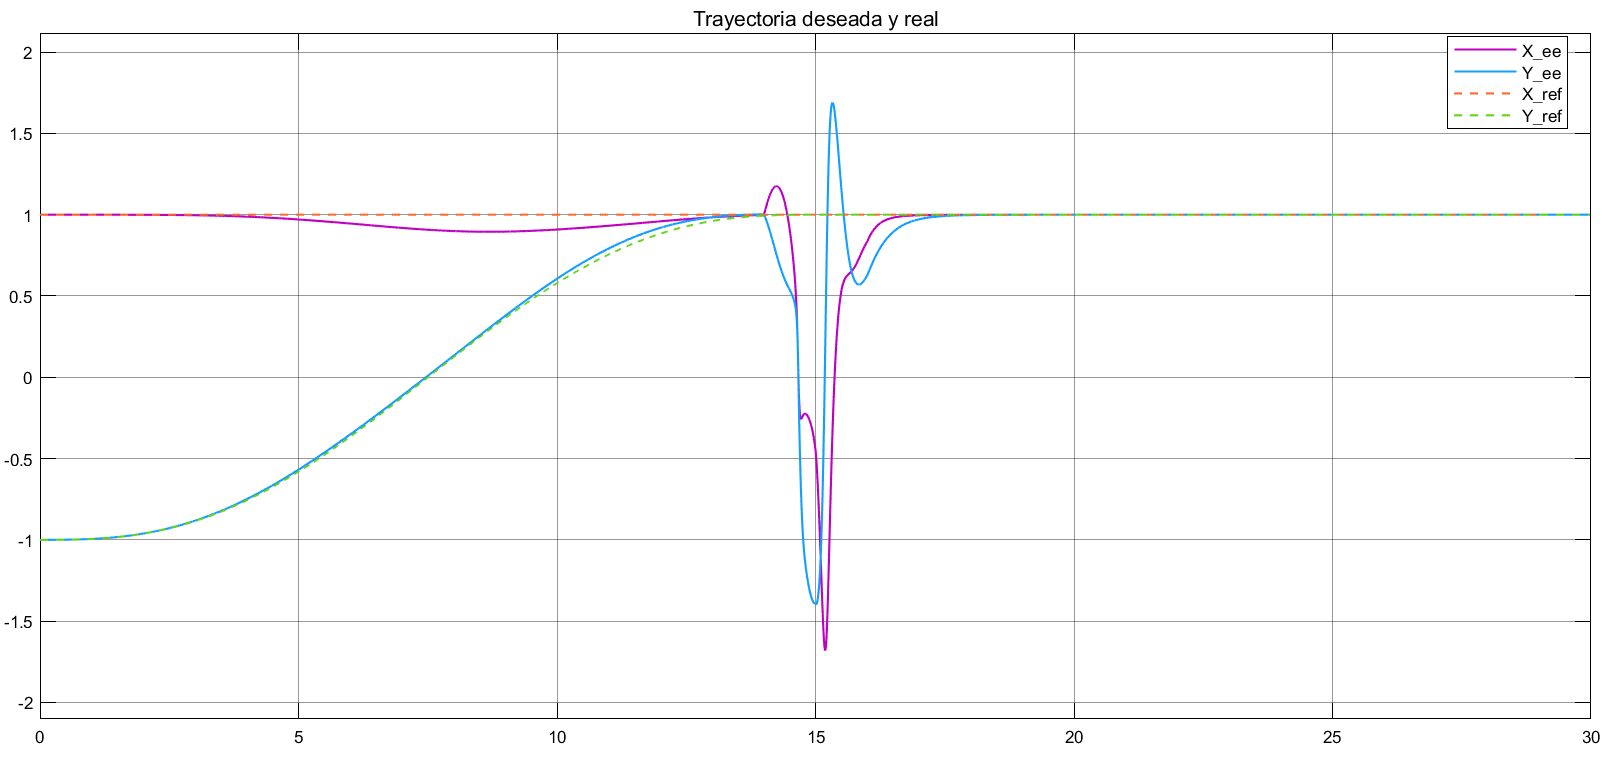
\includegraphics[width=0.8\linewidth]{ImagenesControl de posición no lineal/1_3_e_b}
	\caption{Posici\'on deseada y real del EE.}	
	\label{fig:aposd}
\end{figure}
\begin{figure}[H]
	\centering
	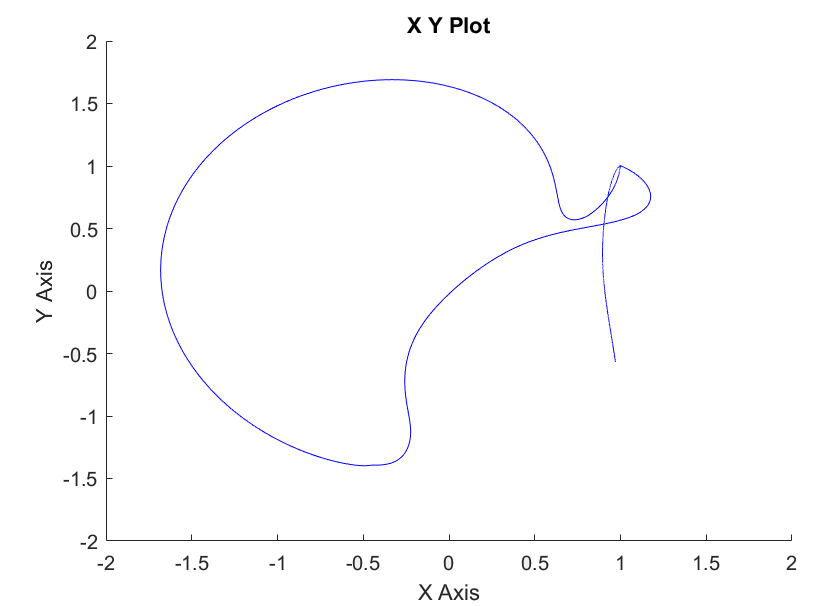
\includegraphics[width=0.5\linewidth]{ImagenesControl de posición no lineal/1_3_e_c}
	\caption{Gr\'afico XY.}	
	\label{fig:axyd}
\end{figure}

%\end{document}


\section{Control de fuerza no lineal}
%\documentclass[a4paper]{article}
\usepackage[utf8]{inputenc}
\usepackage[spanish, es-tabla, es-noshorthands]{babel}
\usepackage[table,xcdraw]{xcolor}
\usepackage[a4paper, footnotesep=1.25cm, headheight=1.25cm, top=2.54cm, left=2.54cm, bottom=2.54cm, right=2.54cm]{geometry}
%\geometry{showframe}

%\usepackage{wrapfig}			%Wrap figure in text
\usepackage[export]{adjustbox}	%Move images
\usepackage{changepage}			%Move tables

\usepackage{tikz}
\usepackage{amsmath}
\usepackage{amsfonts}
\usepackage{amssymb}
\usepackage{float}
\usepackage{graphicx}
\usepackage{caption}
\usepackage{subcaption}
\usepackage{multicol}
\usepackage{multirow}
\usepackage{wrapfig}
\setlength{\doublerulesep}{\arrayrulewidth}
\usepackage{booktabs}
\usepackage[numbib, nottoc, notlot, notlof]{tocbibind}

\usepackage{hyperref}
\hypersetup{
    colorlinks=true,
    linkcolor=blue,
    filecolor=magenta,      
    urlcolor=blue,
    citecolor=blue,    
}

%Change Font Size

% #1 = size, #2 = text
\newcommand{\setparagraphsize}[2]{{\fontsize{#1}{6}\selectfont#2 \par}}		%Cambia el size de todo el parrafo
\newcommand{\setlinesize}[2]{{\fontsize{#1}{6}\selectfont#2}}				%Cambia el font de una oración

\newcommand{\note}[1]{
	\begin{center}
		\huge{ \textcolor{red}{#1} }
	\end{center}
}

%FONTS (IMPORTANTE): Compilar en XeLaTex o LuaLaTeX
\usepackage{anyfontsize}	%Font size
\usepackage{fontspec}		%Font type

\usepackage{etoolbox}
\usepackage{todonotes}

\newcommand{\observacion}[2]{  \ifnumequal{1}{#1}{ { \todo[inline,backgroundcolor=red!25,bordercolor=red!100]{\textbf{Observación: #2}} } }{  }  }

\setcounter{topnumber}{2}
\setcounter{bottomnumber}{2}
\setcounter{totalnumber}{4}
\renewcommand{\topfraction}{0.85}
\renewcommand{\bottomfraction}{0.85}
\renewcommand{\textfraction}{0.15}
\renewcommand{\floatpagefraction}{0.8}
\renewcommand{\textfraction}{0.1}
\setlength{\floatsep}{5pt plus 2pt minus 2pt}
\setlength{\textfloatsep}{5pt plus 2pt minus 2pt}
\setlength{\intextsep}{5pt plus 2pt minus 2pt}

\newcommand{\quotes}[1]{``#1''}
\usepackage{array}
\newcolumntype{C}[1]{>{\centering\let\newline\\\arraybackslash\hspace{0pt}}m{#1}}
\usepackage[american]{circuitikz}
\usetikzlibrary{calc}
\usepackage{fancyhdr}
\usepackage{units} 

\graphicspath{{../Control de posición no lineal/}{../Control de fuerza no lineal/}{../Control híbrido no lineal/}{../Referencias/}{../Deducción de modelo/}{../Conclusiones/}}

\pagestyle{fancy}
\fancyhf{}
\lhead{22.99 - Automación Industrial}
\rhead{Lambertucci, Londero B., Maselli, Mechoulam}
\rfoot{Página \thepage}

%Items con bullets y no cuadrados
\renewcommand{\labelitemi}{\textbullet }


%\begin{document}

\subsection{Caracterización del problema}
A continuación se presenta el desarrollo de un control de fuerzas no lineal. Para ello un aspecto fundamental el modelo de las fuerzas del sistema que interaccionan con el actuador.

En este caso, la fuerza consiste en la pared que trabaja como obstáculo. La fuerza de reacción entre el EE y la pared es aquella definida por:
\begin{equation}
f_r = k_e \cdot d \ \hat{n}
\label{eq:fuerza_pared}
\end{equation}

La Ecuación (\ref{eq:fuerza_pared}) es una fuerza proporcional a la distancia y normal a la superficie de la pared. Esta es nula mientras el EE no se encuentre en contacto con la pared y no nula en caso de estarlo.

\subsection{Esquema de control propuesto}
El esquema de control propuesto es nuevamente una linealización por realimentación de la siguiente manera:

\begin{figure}[H]
	\centering
	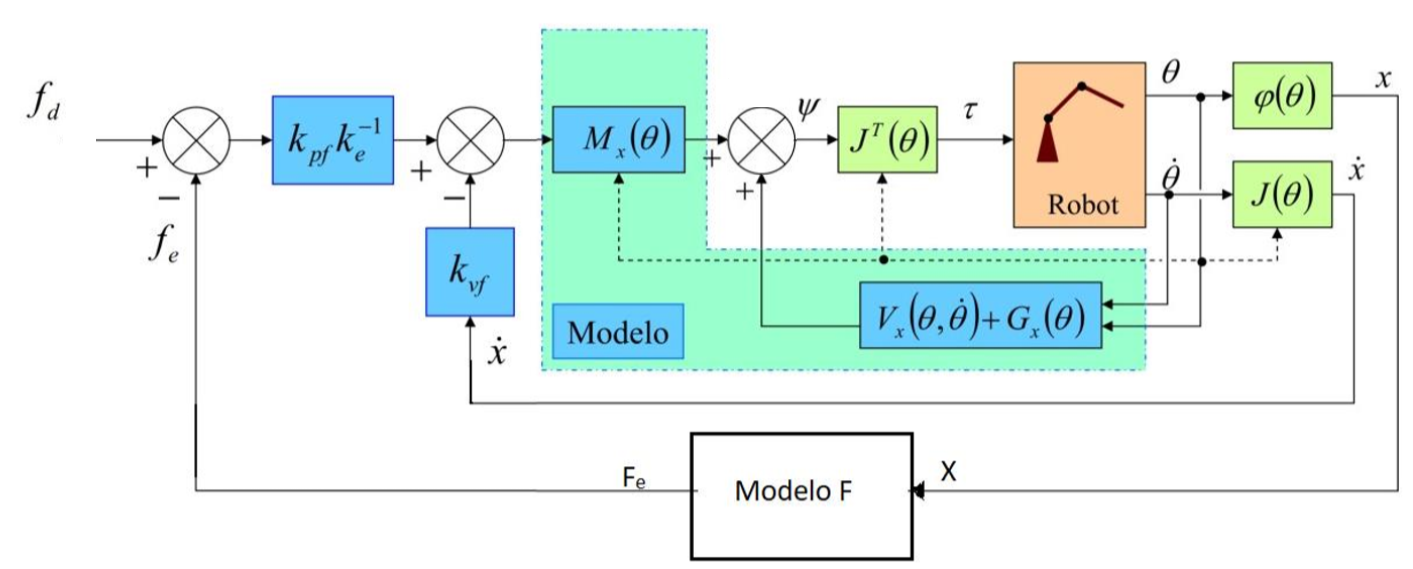
\includegraphics[width=0.8\linewidth]{ImagenesControl de fuerza no lineal/controlf}
	\caption{Topología del control de fuerza no lineal.}	
	\label{fig:control_f_modelo}
\end{figure}

\observacion{\verObs}{HABLAR DE VALORES DE GANANCIAS}

Nuevamente y de manera análoga lo presentado en las Secciones (\ref{sec:posic}) y (\ref{sec:fuerza}), se utilizó el método de Ziegler-Nichols. De esta forma, los valores obtenidos fueron:
\begin{itemize}
	\item Kv = [139 0;0 139].
	\item Kp = [420 0; 0 420].
\end{itemize}

\subsection{Resultados}
Nuevamente se realizó el simulink del sistema, obteniendo así los gráficos que se presentan a continuación.

Algo característico que tiene este control de fuerzas es que, debido a que no hay información provista como referencia de posición, el manipulador se mueve hasta encontrarse cerca de la pared. Luego realiza una breve oscilación sobre el obstáculo hasta llegar a un estado permanente en el cual el manipulador está aplicando la fuerza comandada por la referencia.

\begin{figure}[H]
	\centering
	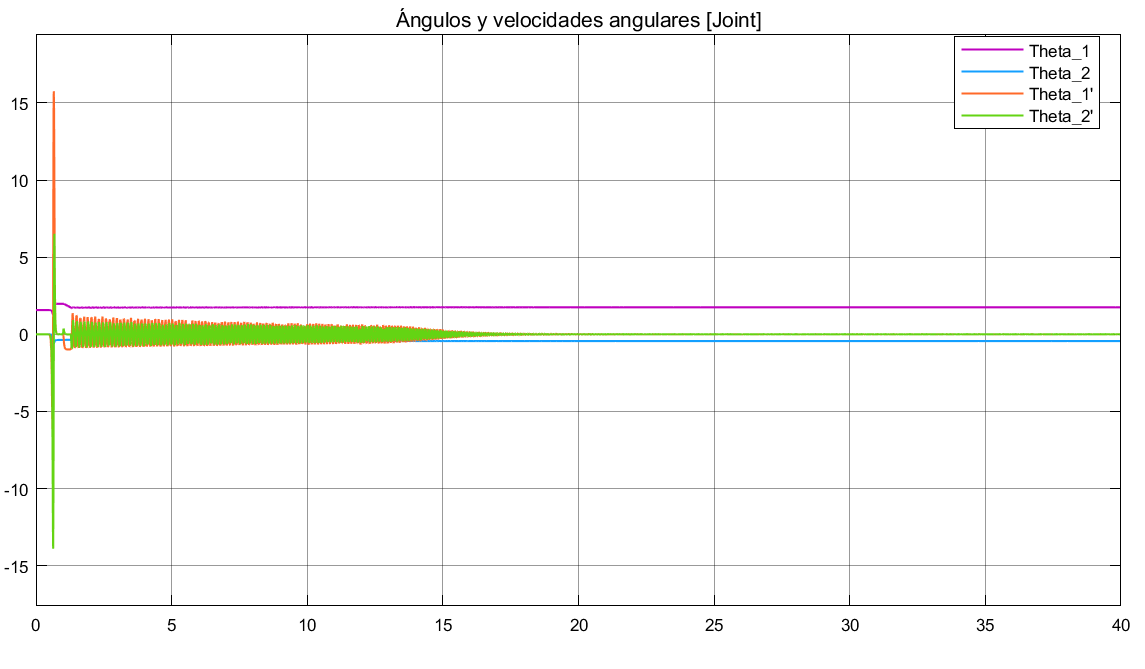
\includegraphics[width=0.8\linewidth]{ImagenesControl de fuerza no lineal/2_3_a}
	\caption{\'Angulos en función del tiempo en espacio joint.}	
	\label{fig:athetas_f}
\end{figure}

Se observa en la Figura (\ref{fig:apos_f}) la leve oscilación del EE al llegar a la pared.

\begin{figure}[H]
	\centering
	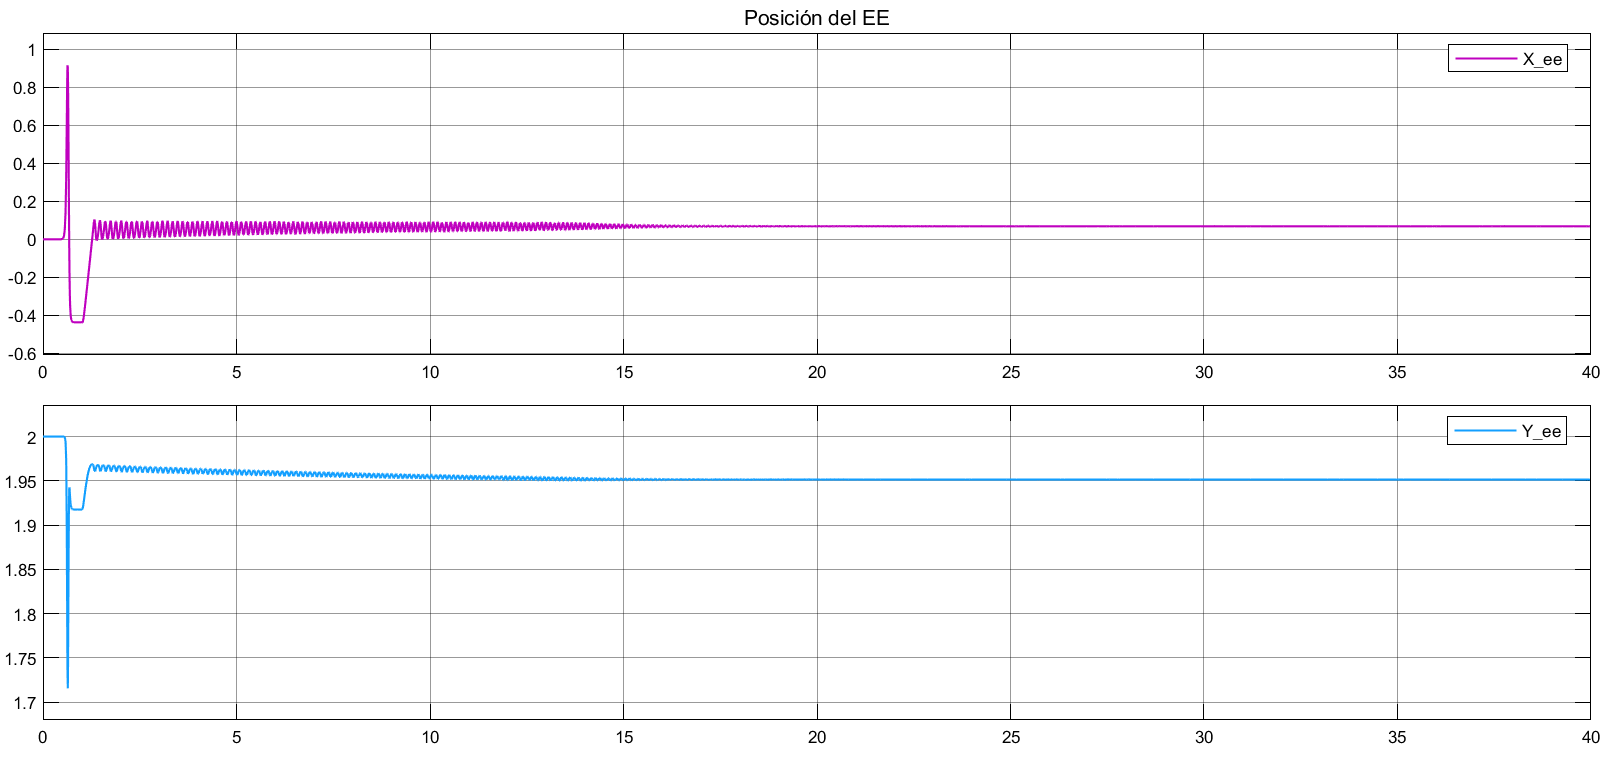
\includegraphics[width=0.8\linewidth]{ImagenesControl de fuerza no lineal/2_3_b}
	\caption{Posición  del EE.}	
	\label{fig:apos_f}
\end{figure}

\begin{figure}[H]
	\centering
	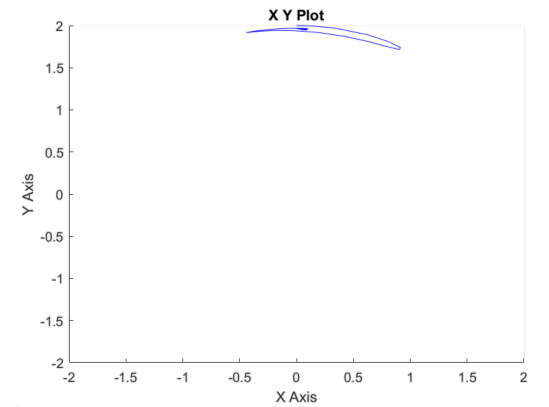
\includegraphics[width=0.5\linewidth]{ImagenesControl de fuerza no lineal/2_3_c}
	\caption{Gráfico XY.}	
	\label{fig:axy_f}
\end{figure}

Cabe mencionar en la Figura (\ref{fig:axy_f}) la función es nula en varios puntos. Esto se debe a que el manipulador no está en contacto con la pared por lo que la misma no aplica una fuerza.

Además se observa como una vez alcanzada la pared y dada una referencia, el EE oscila levemente en torno a la referencia hasta establecerse.

\begin{figure}[H]
	\centering
	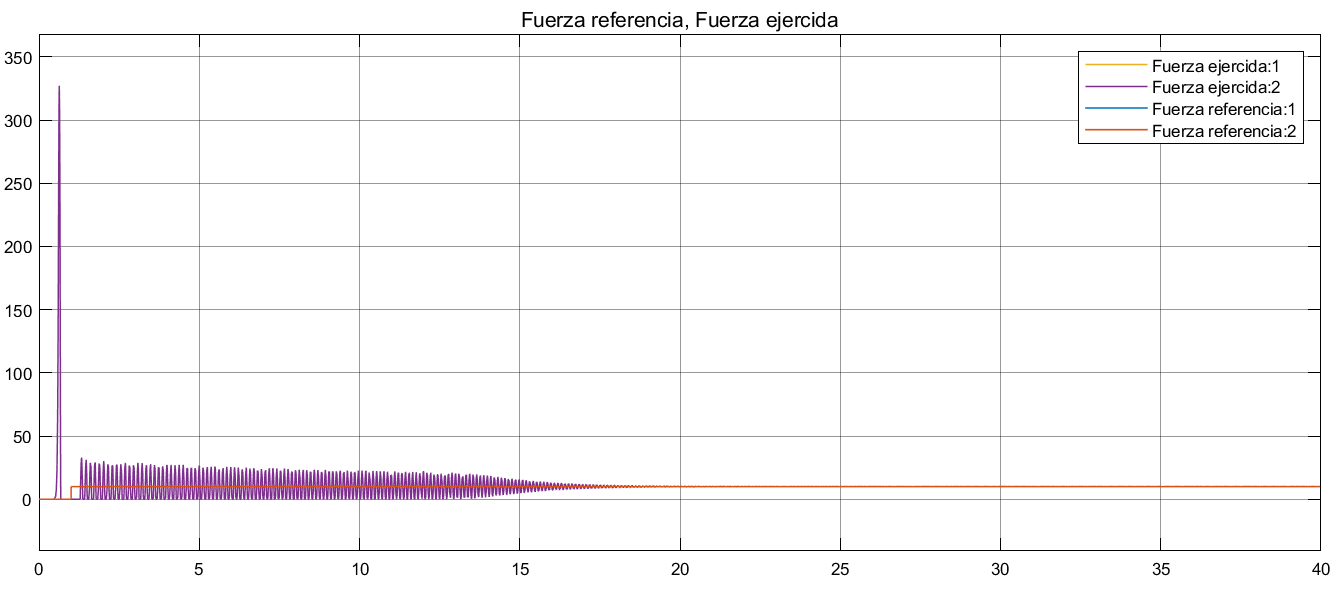
\includegraphics[width=0.8\linewidth]{ImagenesControl de fuerza no lineal/2_3_e}
	\caption{Fuerzas de referencia y ejercida.}	
	\label{fig:af_f}
\end{figure}

También se le incluyó un disturbio a la planta tanto en posición como en velocidad. Se puede ver en la Figura (\ref{fig:athetasd_f}) como el momento en el que se le aplica el disturbio a la planta las variables de estado se estabilizan nuevamente.
\begin{figure}[H]
	\centering
	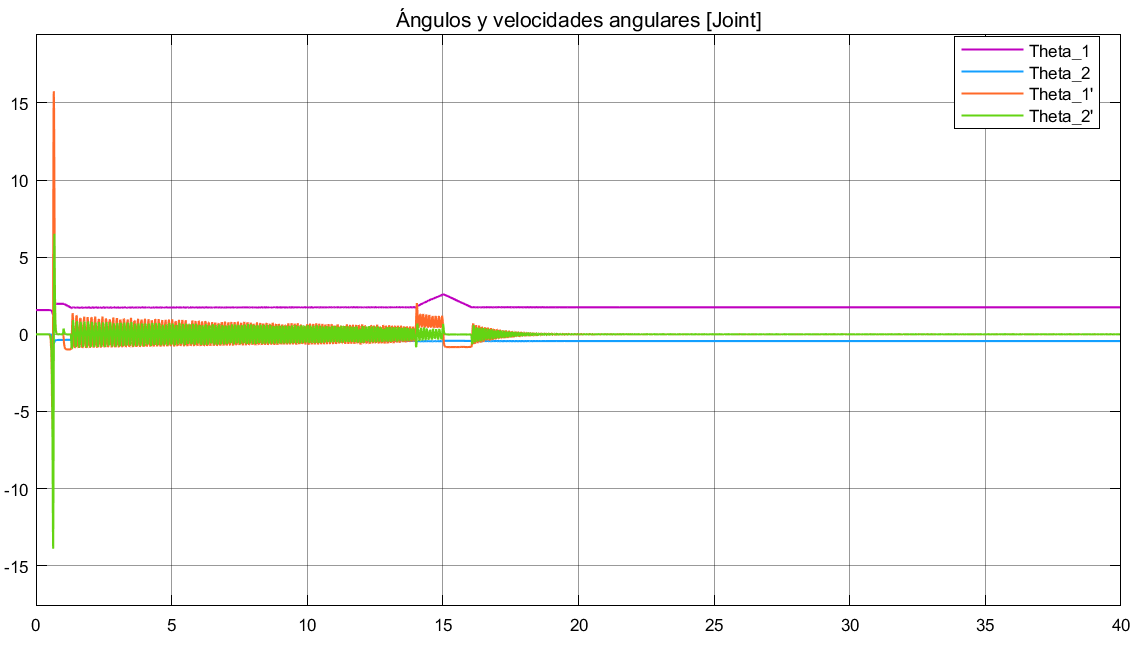
\includegraphics[width=0.8\linewidth]{ImagenesControl de fuerza no lineal/2_3_f_a}
	\caption{Ángulos en función del tiempo en espacio joint.}	
	\label{fig:athetasd_f}
\end{figure}

Luego se muestra el movimiento del EE.
\begin{figure}[H]
	\centering
	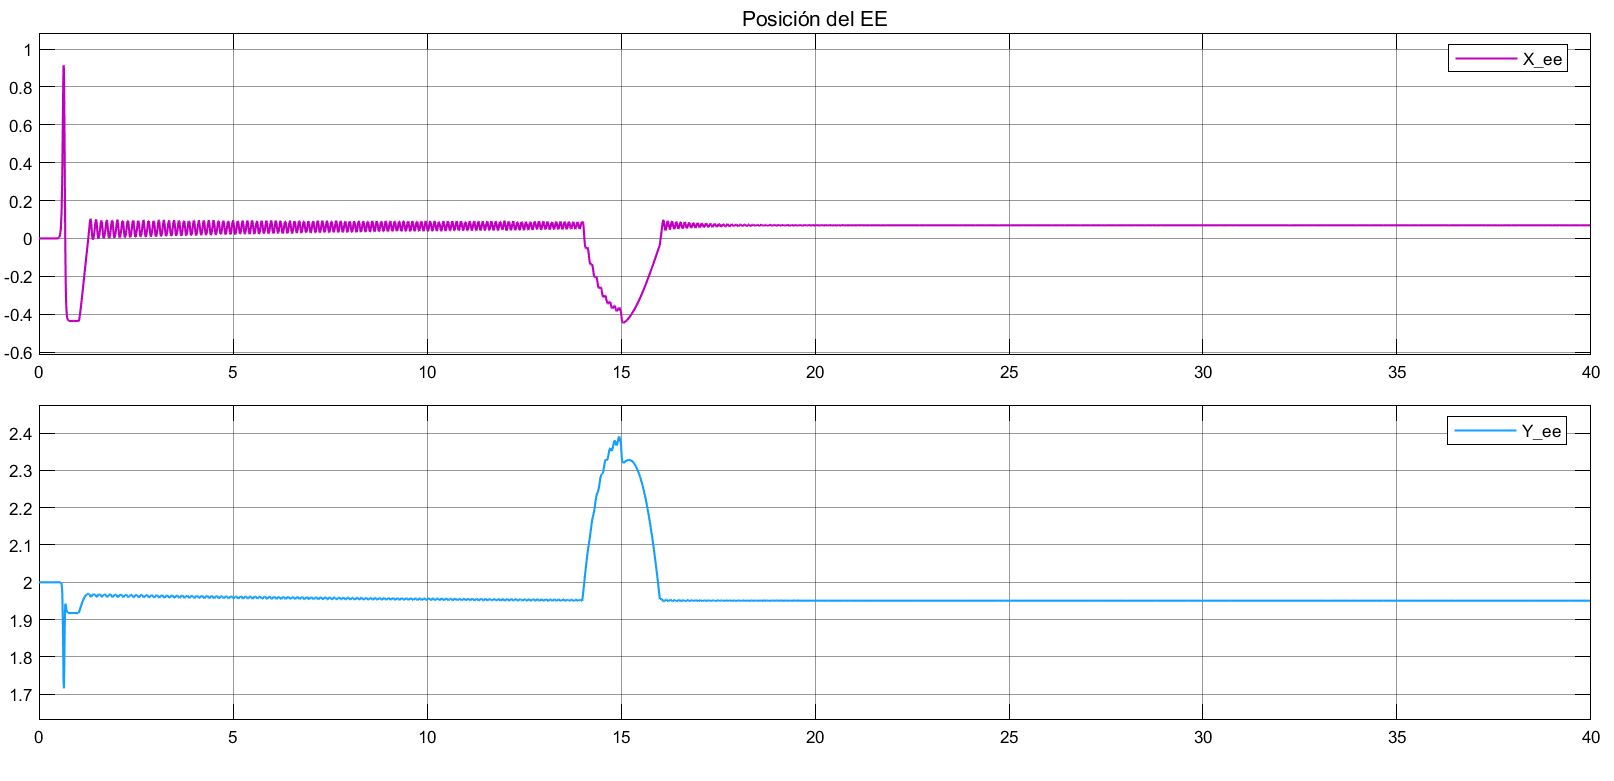
\includegraphics[width=0.8\linewidth]{ImagenesControl de fuerza no lineal/2_3_f_b}
	\caption{Posición del EE.}	
	\label{fig:aposd_f}
\end{figure}

\begin{figure}[H]
	\centering
	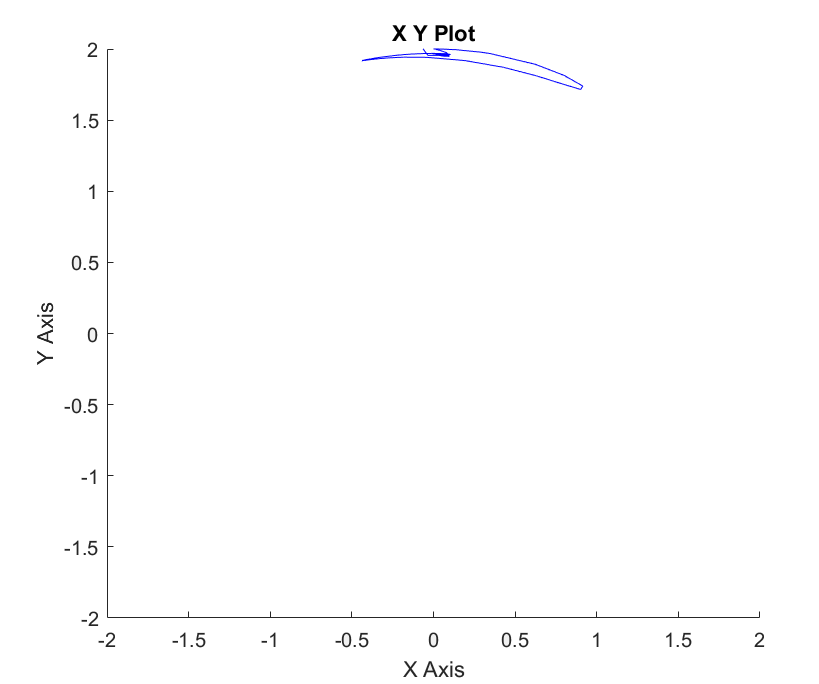
\includegraphics[width=0.5\linewidth]{ImagenesControl de fuerza no lineal/2_3_f_c}
	\caption{Gráfico XY.}	
	\label{fig:bxyd_f}
\end{figure}

Finalmente se observa un gráfico similar al de fuerzas anterior, con la diferencia de que se hace nulo el valor de la fuerza aplicada en el segundo 15. 

En dicho instante es el EE se despega completamente de la pared para luego volver a la misma. Es así que se establece en el régimen permanente nuevamente.

\begin{figure}[H]
	\centering
	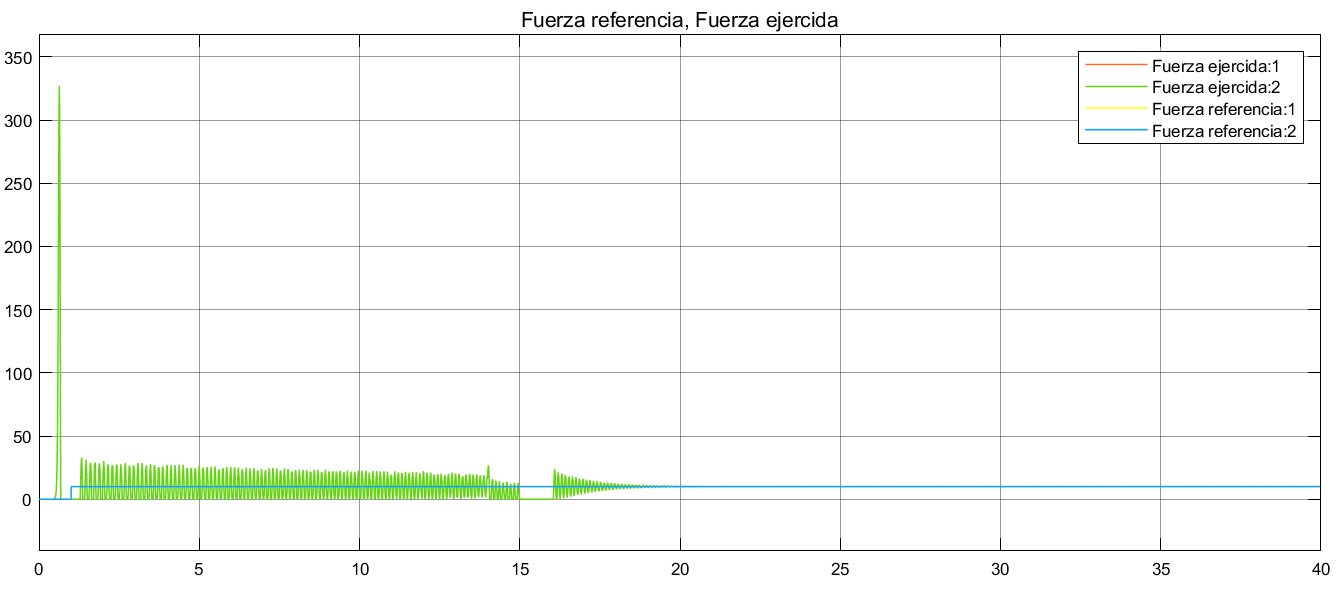
\includegraphics[width=0.8\linewidth]{ImagenesControl de fuerza no lineal/2_3_f_e}
	\caption{Fuerza deseada y real.}	
	\label{fig:bfd_f}
\end{figure}
%\end{document}


\section{Control híbrido no lineal}
%\documentclass[a4paper]{article}
\usepackage[utf8]{inputenc}
\usepackage[spanish, es-tabla, es-noshorthands]{babel}
\usepackage[table,xcdraw]{xcolor}
\usepackage[a4paper, footnotesep=1.25cm, headheight=1.25cm, top=2.54cm, left=2.54cm, bottom=2.54cm, right=2.54cm]{geometry}
%\geometry{showframe}

%\usepackage{wrapfig}			%Wrap figure in text
\usepackage[export]{adjustbox}	%Move images
\usepackage{changepage}			%Move tables

\usepackage{tikz}
\usepackage{amsmath}
\usepackage{amsfonts}
\usepackage{amssymb}
\usepackage{float}
\usepackage{graphicx}
\usepackage{caption}
\usepackage{subcaption}
\usepackage{multicol}
\usepackage{multirow}
\usepackage{wrapfig}
\setlength{\doublerulesep}{\arrayrulewidth}
\usepackage{booktabs}
\usepackage[numbib, nottoc, notlot, notlof]{tocbibind}

\usepackage{hyperref}
\hypersetup{
    colorlinks=true,
    linkcolor=blue,
    filecolor=magenta,      
    urlcolor=blue,
    citecolor=blue,    
}

%Change Font Size

% #1 = size, #2 = text
\newcommand{\setparagraphsize}[2]{{\fontsize{#1}{6}\selectfont#2 \par}}		%Cambia el size de todo el parrafo
\newcommand{\setlinesize}[2]{{\fontsize{#1}{6}\selectfont#2}}				%Cambia el font de una oración

\newcommand{\note}[1]{
	\begin{center}
		\huge{ \textcolor{red}{#1} }
	\end{center}
}

%FONTS (IMPORTANTE): Compilar en XeLaTex o LuaLaTeX
\usepackage{anyfontsize}	%Font size
\usepackage{fontspec}		%Font type

\usepackage{etoolbox}
\usepackage{todonotes}

\newcommand{\observacion}[2]{  \ifnumequal{1}{#1}{ { \todo[inline,backgroundcolor=red!25,bordercolor=red!100]{\textbf{Observación: #2}} } }{  }  }

\setcounter{topnumber}{2}
\setcounter{bottomnumber}{2}
\setcounter{totalnumber}{4}
\renewcommand{\topfraction}{0.85}
\renewcommand{\bottomfraction}{0.85}
\renewcommand{\textfraction}{0.15}
\renewcommand{\floatpagefraction}{0.8}
\renewcommand{\textfraction}{0.1}
\setlength{\floatsep}{5pt plus 2pt minus 2pt}
\setlength{\textfloatsep}{5pt plus 2pt minus 2pt}
\setlength{\intextsep}{5pt plus 2pt minus 2pt}

\newcommand{\quotes}[1]{``#1''}
\usepackage{array}
\newcolumntype{C}[1]{>{\centering\let\newline\\\arraybackslash\hspace{0pt}}m{#1}}
\usepackage[american]{circuitikz}
\usetikzlibrary{calc}
\usepackage{fancyhdr}
\usepackage{units} 

\graphicspath{{../Control de posición no lineal/}{../Control de fuerza no lineal/}{../Control híbrido no lineal/}{../Referencias/}{../Deducción de modelo/}{../Conclusiones/}}

\pagestyle{fancy}
\fancyhf{}
\lhead{22.99 - Automación Industrial}
\rhead{Lambertucci, Londero B., Maselli, Mechoulam}
\rfoot{Página \thepage}

%Items con bullets y no cuadrados
\renewcommand{\labelitemi}{\textbullet }


%\begin{document}

\subsection{XXX}

%\end{document}


\section{Conclusiones}
Hubo la oportunidad de desarrollar analíticamente la mecánica del manipulador propuesto por la cátedra, obteniendo a través del método de Lagrange el vector de torques, al igual que por propagación de velocidades la matriz jacobiana. Parámetros sumamente importantes para la siguiente actividad, la cual fue llevar a cabo diversos tipos de control, tanto de posición y fuerzo e incluso uno híbrido el cual incluía tanto posición como fuerza.

 Se exploraron varias topologías de control no lineal, como puede ser la linealización por punto de equilibrio variable, y la linealización por realimentación. La utilizada fue la linealización por realimetnación debido al amplio conocimiento que se tiene sobre la planta. 

Se profundizó en el uso de simulink  al igual que un aprendizaje en el uso del toolbox de robotics de Peter Corke, una gran herramienta para la simulación de manipuladores. 

Finalmente se observó como era la reacción de los distintos tipos de control ante disturbios en la planta.
Y como estos volvían a sus señales respectivas de referencia.

%\newpage
%\documentclass[a4paper]{article}
\usepackage[utf8]{inputenc}
\usepackage[spanish, es-tabla, es-noshorthands]{babel}
\usepackage[table,xcdraw]{xcolor}
\usepackage[a4paper, footnotesep=1.25cm, headheight=1.25cm, top=2.54cm, left=2.54cm, bottom=2.54cm, right=2.54cm]{geometry}
%\geometry{showframe}

%\usepackage{wrapfig}			%Wrap figure in text
\usepackage[export]{adjustbox}	%Move images
\usepackage{changepage}			%Move tables

\usepackage{tikz}
\usepackage{amsmath}
\usepackage{amsfonts}
\usepackage{amssymb}
\usepackage{float}
\usepackage{graphicx}
\usepackage{caption}
\usepackage{subcaption}
\usepackage{multicol}
\usepackage{multirow}
\usepackage{wrapfig}
\setlength{\doublerulesep}{\arrayrulewidth}
\usepackage{booktabs}
\usepackage[numbib, nottoc, notlot, notlof]{tocbibind}

\usepackage{hyperref}
\hypersetup{
    colorlinks=true,
    linkcolor=blue,
    filecolor=magenta,      
    urlcolor=blue,
    citecolor=blue,    
}

%Change Font Size

% #1 = size, #2 = text
\newcommand{\setparagraphsize}[2]{{\fontsize{#1}{6}\selectfont#2 \par}}		%Cambia el size de todo el parrafo
\newcommand{\setlinesize}[2]{{\fontsize{#1}{6}\selectfont#2}}				%Cambia el font de una oración

\newcommand{\note}[1]{
	\begin{center}
		\huge{ \textcolor{red}{#1} }
	\end{center}
}

%FONTS (IMPORTANTE): Compilar en XeLaTex o LuaLaTeX
\usepackage{anyfontsize}	%Font size
\usepackage{fontspec}		%Font type

\usepackage{etoolbox}
\usepackage{todonotes}

\newcommand{\observacion}[2]{  \ifnumequal{1}{#1}{ { \todo[inline,backgroundcolor=red!25,bordercolor=red!100]{\textbf{Observación: #2}} } }{  }  }

\setcounter{topnumber}{2}
\setcounter{bottomnumber}{2}
\setcounter{totalnumber}{4}
\renewcommand{\topfraction}{0.85}
\renewcommand{\bottomfraction}{0.85}
\renewcommand{\textfraction}{0.15}
\renewcommand{\floatpagefraction}{0.8}
\renewcommand{\textfraction}{0.1}
\setlength{\floatsep}{5pt plus 2pt minus 2pt}
\setlength{\textfloatsep}{5pt plus 2pt minus 2pt}
\setlength{\intextsep}{5pt plus 2pt minus 2pt}

\newcommand{\quotes}[1]{``#1''}
\usepackage{array}
\newcolumntype{C}[1]{>{\centering\let\newline\\\arraybackslash\hspace{0pt}}m{#1}}
\usepackage[american]{circuitikz}
\usetikzlibrary{calc}
\usepackage{fancyhdr}
\usepackage{units} 

\graphicspath{{../Control de posición no lineal/}{../Control de fuerza no lineal/}{../Control híbrido no lineal/}{../Referencias/}{../Deducción de modelo/}{../Conclusiones/}}

\pagestyle{fancy}
\fancyhf{}
\lhead{22.99 - Automación Industrial}
\rhead{Lambertucci, Londero B., Maselli, Mechoulam}
\rfoot{Página \thepage}

%Items con bullets y no cuadrados
\renewcommand{\labelitemi}{\textbullet }


\begin{document}

\begin{flushleft}
\begin{thebibliography}{9}

\bibitem{ref:final}
\quotes{Limit switch - Wikipedia}, En.wikipedia.org, 2021. [Online]. Disponible: \href{https://en.wikipedia.org/wiki/Limit\_switch}{https://en.wikipedia.org/wiki/Limit\_switch}. [Accedido: 28 Agosto 2021].

\end{thebibliography}
\end{flushleft}

\end{document}


\end{document}
